\documentclass[10pt]{article}
\usepackage[letterpaper,text={6.5in,8.7in},centering]{geometry}
\usepackage{curves}
\usepackage{epic,eepic,color}
%\usepackage[usenames,dvipsnames,svgnames,table]{xcolor}
\usepackage{amssymb,amsmath,times,subfigure,graphicx,theorem}
\usepackage{alltt}
%\usepackage{warmread}
%\usepackage[all,import]{xy}
%\usepackage{eepic}

\newcommand{\norm}[1]{\ensuremath{\left\| #1 \right\|}}
\newcommand{\abs}[1]{\ensuremath{\left| #1 \right|}}
\newcommand{\bracket}[1]{\ensuremath{\left[ #1 \right]}}
\newcommand{\braces}[1]{\ensuremath{\left\{ #1 \right\}}}
\newcommand{\parenth}[1]{\ensuremath{\left( #1 \right)}}
\newcommand{\ip}[1]{\ensuremath{\langle #1 \rangle}}
\newcommand{\refeqn}[1]{(\ref{eqn:#1})}
\newcommand{\reffig}[1]{Fig. \ref{fig:#1}}
\newcommand{\tr}[1]{\mbox{tr}\ensuremath{\negthickspace\bracket{#1}}}
\newcommand{\deriv}[2]{\ensuremath{\frac{\partial #1}{\partial #2}}}
\newcommand{\SO}{\ensuremath{\mathrm{SO(3)}}}
\newcommand{\T}{\ensuremath{\mathrm{T}}}
\newcommand{\so}{\ensuremath{\mathfrak{so}(3)}}
\newcommand{\SE}{\ensuremath{\mathrm{SE(3)}}}
\newcommand{\se}{\ensuremath{\mathfrak{se}(3)}}
\renewcommand{\Re}{\ensuremath{\mathbb{R}}}
\renewcommand{\S}{\ensuremath{\mathbb{S}}}
\newcommand{\aSE}[2]{\ensuremath{\begin{bmatrix}#1&#2\\0&1\end{bmatrix}}}
\newcommand{\ase}[2]{\ensuremath{\begin{bmatrix}#1&#2\\0&0\end{bmatrix}}}
\newcommand{\D}{\ensuremath{\mathbf{D}}}
\newcommand{\pair}[1]{\ensuremath{\left\langle #1 \right\rangle}}
\newcommand{\met}[1]{\ensuremath{\langle\!\langle #1 \rangle\!\rangle}}
\newcommand{\Ad}{\ensuremath{\mathrm{Ad}}}
\newcommand{\ad}{\ensuremath{\mathrm{ad}}}
\newcommand{\g}{\ensuremath{\mathfrak{g}}}

\renewcommand{\baselinestretch}{1.2}
\date{}

\renewcommand{\thesubsection}{\arabic{subsection}. }
\renewcommand{\thesubsubsection}{\arabic{subsection}.\arabic{subsubsection} }

\theoremstyle{plain}\theorembodyfont{\normalfont}
\newtheorem{prob}{Problem}[section]
%\renewcommand{\theprob}{\arabic{section}.\arabic{prob}}
\renewcommand{\theprob}{\arabic{prob}}

\newenvironment{subprob}%
{\renewcommand{\theenumi}{\alph{enumi}}\renewcommand{\labelenumi}{(\theenumi)}\begin{enumerate}}%
{\end{enumerate}}%


%1: Explain the Newtonian gravitational force and gravitational potential between particles
%2: Analyze the characteristics of circular, elliptic, parabolic and hyperbolic orbits in a two-dimensional plane
%3: Describe the geometry of an orbit in a three-dimensional space from orbital elements
%4: Find an orbital position as a function of time


\begin{document}


\vspace*{1cm}

\pagestyle{empty}
\centerline{\LARGE{ MAE3145: Midterm Exam (Practice)}}
\vspace*{0.5cm}
\centerline{\Large October 26, 2016}%\\%\vspace*{0.5cm}

\vspace*{6cm}

\centerline{
\begin{tabular}{lll}
\hspace*{5cm}, & \hspace*{5cm}. & \hspace*{4cm}\\\hline
Last Name & First Name & Student ID
\end{tabular}}

\vspace*{6cm}

\centerline{
\begin{tabular}{|c|c|c|c|}\hline
Prob. 1 & Prob. 2 & Prob. 3  & Total \\
(3) & (16) & (15) & (34) \\ \hline
\hspace*{2.2cm} & \hspace*{2.2cm} & \hspace*{2.2cm} & \hspace*{2.6cm} \\
&&&\\
&&&\\\hline
\end{tabular}}

$ $\clearpage\newpage$ $

\renewcommand{\thepage}{\arabic{page}/4}
\clearpage\newpage\setcounter{page}{1}\pagestyle{plain}

\renewcommand{\theprob}{\arabic{prob} \textit{(3pt)}}
\begin{prob}
Mark whether each statement written in \textit{italic font} is True or False.
\begin{subprob}


\item \textit{The orbital speed of the Mars around the Sun is greater than that of the Earth.} [True, False]
%
%\vfill
%
%\item Consider the following two spacecraft, namely $A$ and $B$ on circular orbits. 
%The orbital radius and the mass of them are denoted by $r_A,m_A$, and $r_B,m_B$, respectively. Suppose that $r_B=2r_A$ and $m_B=3m_A$. Then, \textit{the gravitational potential energy of Spacecraft $A$ is greater than that of Spacecraft $B$}. [True, False]\\
%(Hint: $U=-\frac{GMm}{r}$)
%
%
%%\vspace*{0.3cm}
%%\centerline{
%%\setlength{\unitlength}{2.5em}\centering\footnotesize
%%\begin{picture}(3,3)(-1.5,-1.5)
%%\put(0,0){\circle*{0.3}}
%%\put(0,0){\circle{1.5}}
%%\put(0,0){\circle{3}}
%%\put(0.6495,0.3750){\circle*{0.1}}
%%\put(1.5,0){\circle*{0.06}}
%%\put(1.6,-0.3){$B$}
%%\put(0.8,0.3){$A$}
%%\put(3,-0.2){\shortstack[c]{$r_B=2r_A$\\$m_B=0.3m_A$}}
%%\end{picture}}
%
%\vfill 
%
%\item For the two spacecraft $A$ and $B$ discussed above at the part (b), \textit{the \underline{specific} orbital energy of Spacecraft $A$ is greater than that of Spacecraft $B$, i.e. $\mathcal{E}_A > \mathcal{E}_B$}. [True, False]
%
%
%\vfill

%\item International space station (ISS) is on a circular orbit at the altitude of $422\,\mathrm{km}$, and GPS satellites are on circular orbits at the altitude of $20200\,\mathrm{km}$. \textit{The specific orbital energy of ISS is greater than GPS satellites, i.e. $\mathcal{E}_{ISS} > \mathcal{E}_{GPS}$}, [True, False]
%
%\vspace*{1cm}
%
%\item \textit{The orbital period of ISS is greater than GPS satellites, i.e. $T_{ISS} > T_{GPS}$}, [True, False]
%
%\vspace*{1cm}

%\item Two circular orbits, namely Orbit 1 and Orbit 2 are illustrated with respect to the geocentric equatorial frame as follows, where gray circles denote the Earth equatorial plane, and the blue circle and the green circle denote the orbital plane for Orbit 1 and Orbit 2, respectively. Note that spacecraft on Orbit 1 is rotating \underline{clockwise}, and spacecraft on Orbit 2 is rotating \underline{counterclockwise}. Then, \textit{the longitude of ascending node of Orbit 1 is greater than Orbit 2, i.e. $\Omega_1 > \Omega_2$.} [True, False]
%
%\renewcommand{\thesubfigure}{}
%\setlength{\unitlength}{0.1\textwidth}
%\begin{figure}[h]
%\centerline{\footnotesize
%	\subfigure[Orbit 1]{\begin{picture}(2.2,2.25)(0,0.05)
%	\put(0,0.395){\includegraphics[width=0.25\textwidth]{prob1c1}}
%	\put(0.2,0.4){$\vec X$}
%	\put(2.5,0.6){$\vec Y$}
%	\put(1.25,2.2){$\vec Z$}
%	\end{picture}}\hspace*{0.2\textwidth}
%	\subfigure[Orbit 2]{\begin{picture}(2.2,2.25)(0,0.05)
%	\put(0,0){\includegraphics[width=0.25\textwidth]{prob1c2}}
%	\put(0.2,0.5){$\vec X$}
%	\put(2.4,0.6){$\vec Y$}
%	\put(1.25,2.3){$\vec Z$}
%	\end{picture}}
%}
%\end{figure}


%\item The Aitken basin is the largest crater on the far side of the Moon. The following two lunar orbits, namely Orbit 1 and Orbit 2 are proposed to generate a topographic map of the Aitken basin, which is denoted by $A$ below. The size and the shape of two orbits are identical, i.e., $a_1=a_2$, $e_1=e_2$, and $T_1=T_2$. Assume that the Moon is not rotating: $A$ is stationary with respect to both orbits. Then, \textit{spacecraft on Orbit 1 can take images of $A$ for a longer time period per each revolution than another spacecraft on Orbit 2}. [True, False]
%
%\definecolor{dunkelmagenta}{rgb}{.3, 0, .3}
%
%
%\vspace*{0.3cm}
%\centerline{
%\setlength{\unitlength}{0.08\textwidth}\centering\footnotesize
%\begin{picture}(3,2)(-1.5,-1)
%\put(0,0){\circle*{0.4}}
%\put(1.0,0){\ellipse{3.0}{2}}
%{\filltype{white}
%\put(0.2,0.0){\circle*{0.06}}}
%\put(0.9,-1.2){\text{Orbit 2}}
%\put(0.25,0.05){$A$}
%\put(-0.25,-0.4){\text{Moon}}
%\put(1.0,-1){\vector(1,0){0}}
%\put(1.0,1){\vector(-1,0){0}}
%\color{blue}\put(-1.0,0){\ellipse{3.0}{2}}
%\put(-1.0,-1){\vector(1,0){0}}
%\put(-1.0,1){\vector(-1,0){0}}
%\put(-1.6,-1.2){\text{Orbit 1}}
%\end{picture}}
%%
%\vspace*{1cm}
%
%\item Ground track of a satellite is the projection of the orbit of the satellite onto the surface of the Earth. Ground tracks for two satellites are illustrated as follows. \textit{The inclination of Satellite 1 is greater than Satellite 2, i.e. $i_1> i_2$}. [True, False]
%
%\centerline{
%\setlength{\unitlength}{0.1\textwidth}\centering
%\begin{picture}(6,3.2)(0,0)\footnotesize
%\put(0,0){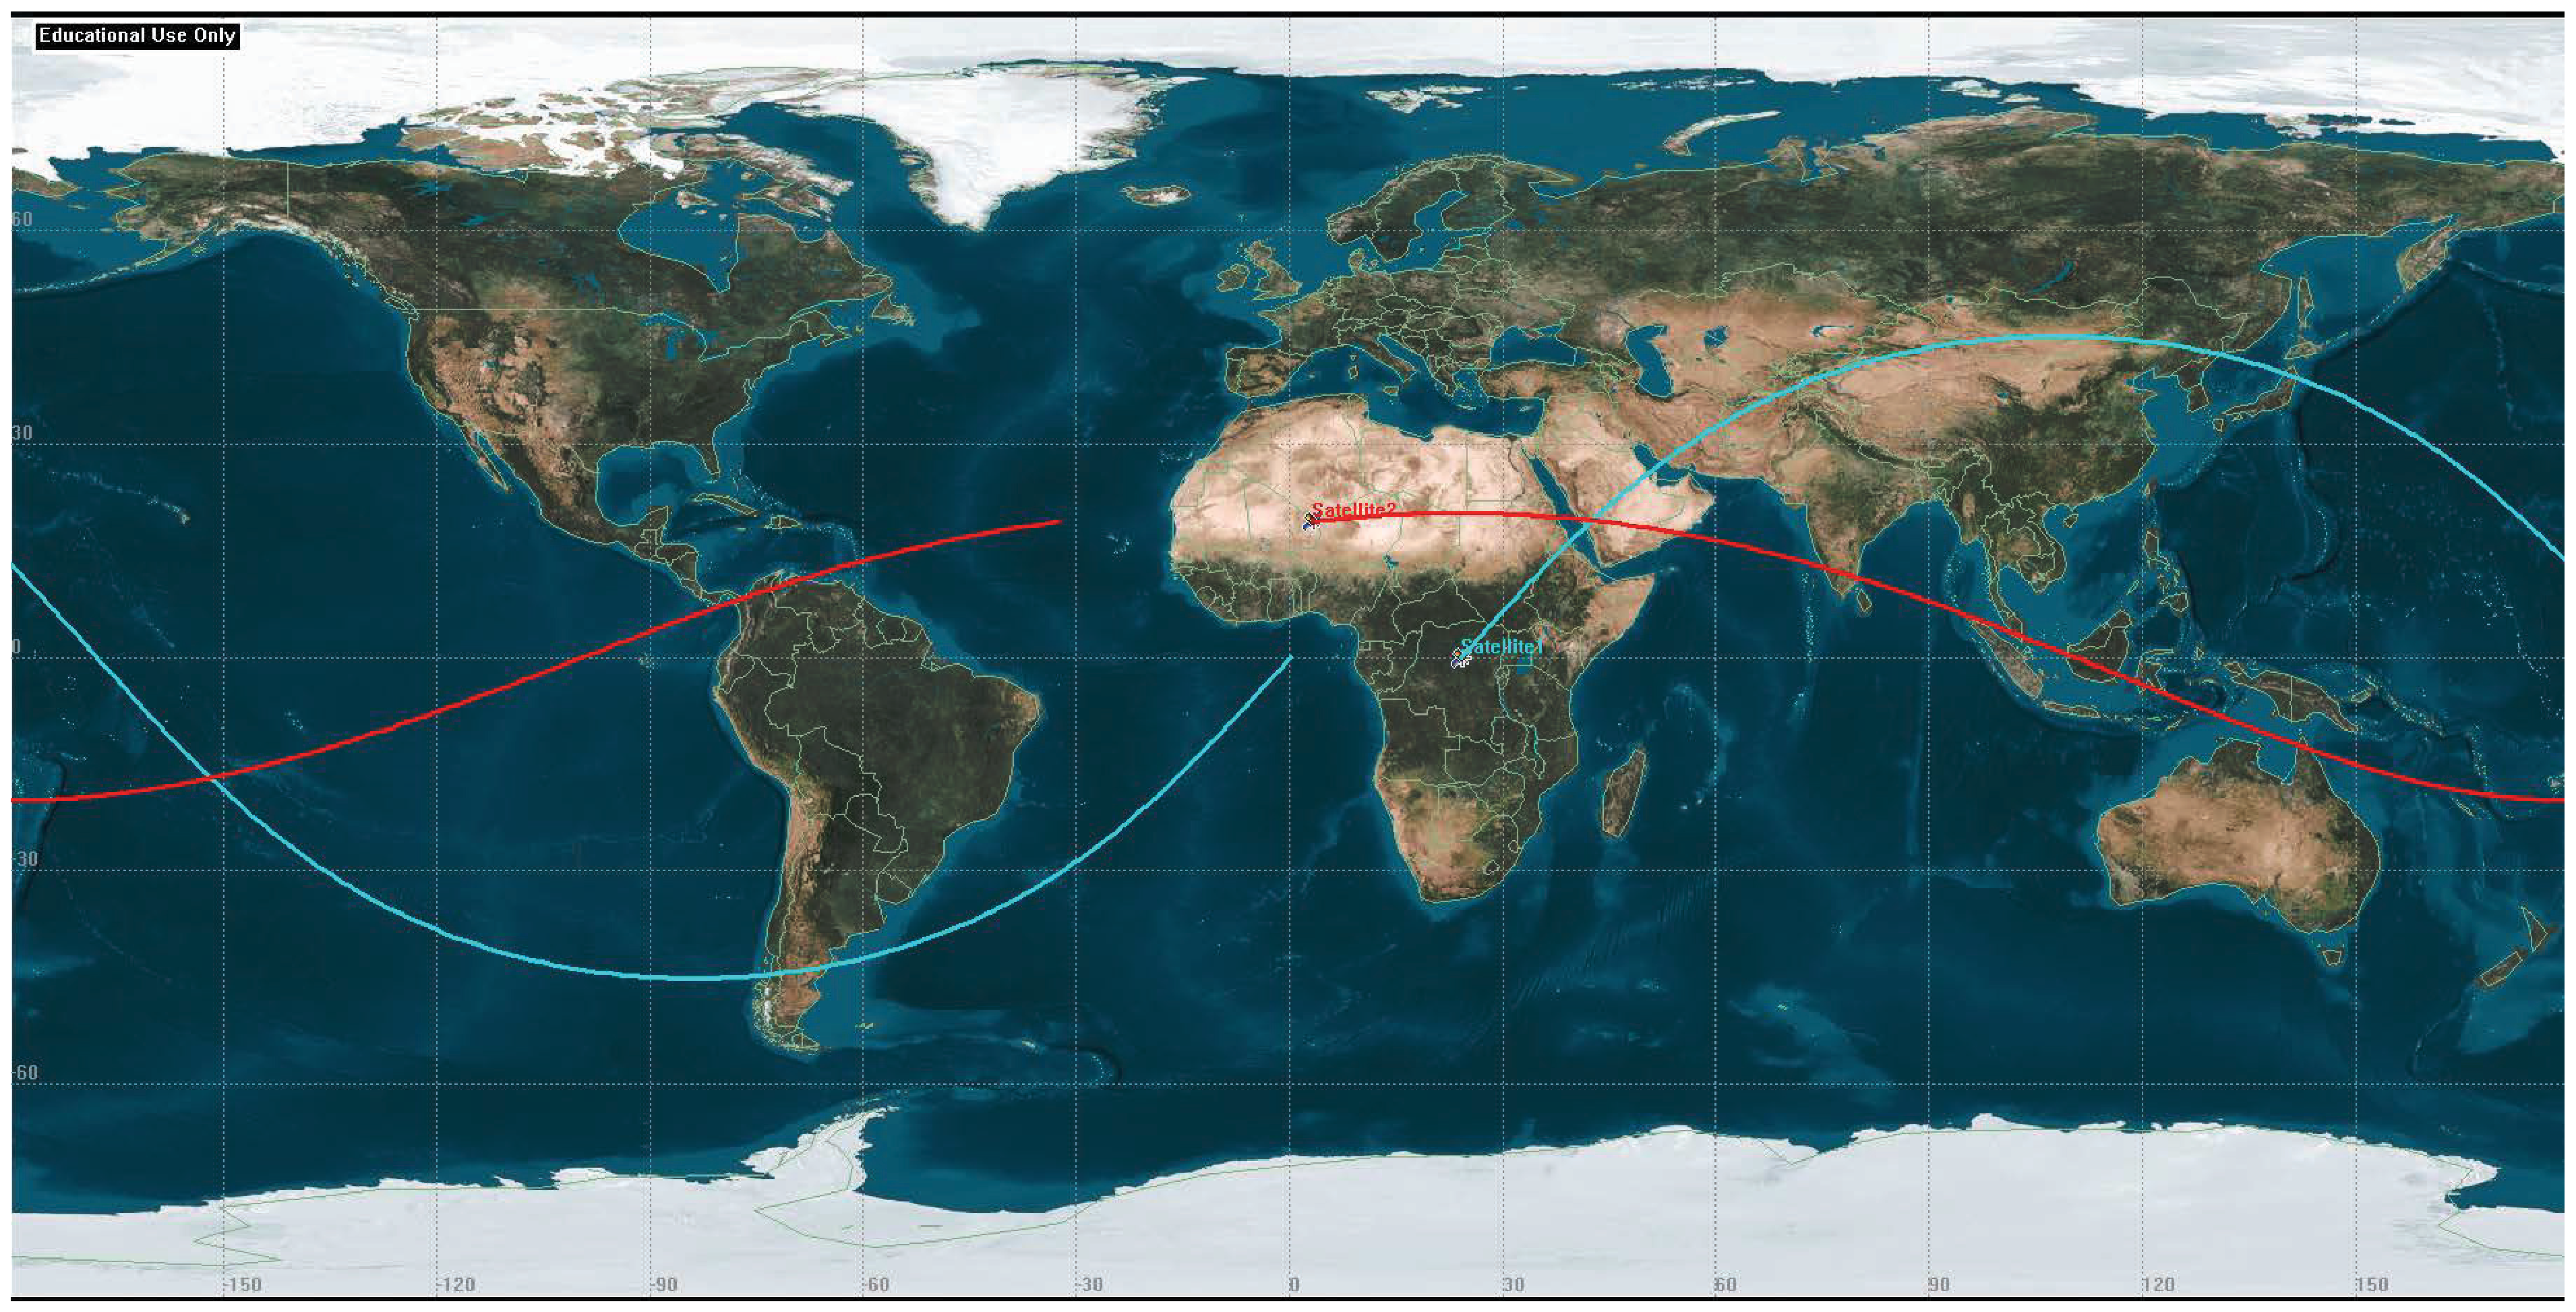
\includegraphics[width=0.60\textwidth]{Prob1.eps}}
%\put(6.1,1.7){Satellite 1 (blue)}
%\put(6.1,1.05){Satellite 2 (red)}
%\end{picture}}
%
%\vspace*{1cm}
%
%\item Since the Earth is rotating, ground track depends on the spin rate of the Earth. \textit{Assuming the ground tracks at (d) are illustrated for one revolution of each satellite, the orbital period of Satellite 1 is greater than Satellite 2, i.e., $T_1 > T_2$}. [True, False]
%
%
%
%%\vspace*{3cm}
%
%
%%\item \textit{Newton's 2nd law of motion is satisfied for any reference frame}. [True, False]
%%\item \textit{The mutual gravitational potential between two point masses is proportional to the distance between them.} [True, False]
%
%%\item \textit{The orbital speed of the Mars around the Sun is greater than that of the Saturn.} [True, False]

\end{subprob}
\end{prob}



%\newpage
%\renewcommand{\theprob}{\arabic{prob} \textit{(12pt)}}
%
%\begin{prob}
%\textbf{(Two-body problem with respect to the inertial frame)}
%The position and the velocity of an asteroid heading toward a planet are measured with respect to an arbitrary $x$-$y$ frame as follows:
%\begin{align*}
%\vec r =[20,\; 15,\; 0]\,\mathrm{km}, \quad \vec v=[-6,\; 0,\; 0] \,\mathrm{km/s}.
%\end{align*}
%%
%\centerline{
%\setlength{\unitlength}{0.04\textwidth}\centering\footnotesize
%\begin{picture}(4,5)(0,-1)
%\put(0,0){\circle*{1}}
%\put(4,3){\circle*{0.2}}
%\put(-2,0){\vector(1,0){7}}
%\put(0,-1){\vector(0,1){5}}
%\put(0,0){\vector(4,3){3.9}}
%\put(4,3){\vector(-1,0){1}}
%\put(5,-0.3){$x$}
%\put(0.2,4){$y$}
%\put(2,1.1){$\vec r$}
%\put(3.5,3.1){$\vec v$}
%\put(-1.4,1.4){\circle*{0.1}}
%\put(-1.8,1.5){$P$}
%\put(0,0){\vector(-1,1){1.35}}
%\put(-1.2,0.5){$\vec r_p$}
%\put(0.5,-0.5){Planet}
%\put(4.2,3.1){Asteroid}
%\end{picture}}
%%
%We wish to determine whether it would hit the planet. The gravitational parameter of the planet is given by {$\underline{ \mu=400\,\mathrm{km^3/s^2}}$}, and the radius of the planet is $R_{\mathrm{planet}}=6\,\mathrm{km}$. 
%
%\begin{subprob}
%\item Find the specific energy $\mathcal{E}$ and the angular momentum $h$.
%\vspace*{3.5cm}
%\item Show that the eccentricity is given by $e=1.0966$, and ALSO show that the asteroid does not hit the planet, i.e., $r_p > R_{\mathrm{planet}}=6\,\mathrm{km}$.
%\vspace*{3.5cm}
%\item We wish to find the point where the asteroid is closest to the planet. Find the \underline{vector} $\vec r_p$ from the center of the planet to the closest point $P$. 
%\end{subprob}
%
%\end{prob}


%\begin{prob}
%\textbf{(Motion with respect to the inertial frame and gravity)} By observation relative to stars, the angular velocity $\omega$ of the line joining the Earth and the Moon is measured as $\omega=2.5\times 10^{-6}\,\mathrm{rad/sec}$. We wish to determine the distance $r$ between the Earth and the Moon using $\omega$ as follows.
%
%The location of the Earth with respect an inertial frame is denoted by $\vec R_1$, and the location of the Moon with respect to the inertial frame is denoted by $\vec R_2$. The relative position of the Moon from the Earth is given by $\vec r = \vec R_2 - \vec R_1$. Let $m_1\in\Re$ and $m_2\in\Re$ be the mass of the Earth and and the mass of the Moon respectively. 
%
%%Define a unit-less mass ratio:
%%\begin{align*}
%%a=\frac{m_2}{m_1+m_2}.
%%\end{align*}
%
%
%\begin{subprob}
%\item Recall that the mass center is given by $\vec R_G = \dfrac{m_1 \vec R_1 + m_2 \vec R_2}{m_1+m_2}$. Show that $\vec R_1$ can be written in terms of $\vec R_G$, and $\vec r$, as
%\begin{align}
%\vec R_1 = \vec R_G + \frac{m_2}{m_1+m_2}\vec r.
%\end{align}
%(Derive the above equation from the definition of $\vec R_G$ and $\vec r$)
%\vspace*{5cm}
%
%\item Assuming that the distance $r$ is fixed, the acceleration of the relative position $\vec r$ is given by the centripetal acceleration, i.e., $\ddot{\vec r}= -\omega^2\vec r$. Using this and (1), show that the distance between the Earth and the Moon can be written as
%\begin{align*}
%r = \parenth{\frac{G(m_1+m_2)}{\omega^2}}^{1/3}.
%\end{align*}
%\end{subprob}
%
%
%
%\end{prob}


\clearpage\newpage
\renewcommand{\theprob}{\arabic{prob} \textit{(16pt)}}
\begin{prob}
\textbf{(Properties of orbit in 2D)} A rocket is fired at the point $B$ on the surface of the Earth. The velocity and the flight path angle of the rocket is given by
\begin{align*}
v=5\,\mathrm{km/s},\quad \gamma= 30^\circ.
\end{align*}
We wish to determine where the rocket would hit on the surface of the Earth. The radius of the Earth and the gravitational parameter are given by
\begin{align*}
R_E=6378\,\mathrm{km},\quad \mu=398,\!600\,\mathrm{km^3/s^2}.
\end{align*}
Throughout this question, ignore the atmospheric drag or the rotation of the Earth.

\vspace*{0.5cm}
\centerline{
\setlength{\unitlength}{0.08\textwidth}\centering\footnotesize
\begin{picture}(6,6)(-3,-3)
\put(0,0){\circle{5.0}}
\put(0,0){\vector(1,0){4}}
\put(0,0){\line(-1,0){3.3}}
\put(0,0){\vector(0,1){3.3}}
\put(0,0){\line(0,-1){3.3}}
\put(2.5,0){\circle*{0.1}}
\put(2.5,0){\vector(2,3){0.8}}
\put(2.5,0){\line(0,1){0.8}}
\put(2.6,0.5){$\gamma$}
\put(3.4,1.1){$v$}
\put(2.6,-.3){$B$}
%\put(0,0){\circle*{3.0}}
%\put(3,0){\circle*{0.2}}
%\put(3,0){\vector(0,1){2}}
%\put(3,0){\vector(-1,0){1}}
%\put(3.1,1.7){$v_\theta$}
%\put(2.1,-0.3){$v_r$}
%\put(3.1,-0.3){$ISS$}
%{\filltype{white}\put(3.0,0){\circle*{0.07}}}
\end{picture}}
\vspace*{0.5cm}


\begin{subprob}
\item Show that $\mathcal{E}=-49.9961\mathrm{km^2/s^2}$, and $h =2.7618\times 10^4\,\mathrm{km^2/s}$.
\vspace*{5cm}
\clearpage\newpage
\item Show that the eccentricity of the rocket is given by $e =0.7211$.
\vfill
\item Find the true anomaly $\theta_B$ of the rocket, when it is fired.
\vfill
\item Find the true anomaly $\theta_H$ of the rocket, when it hits the surface of the Earth.
\vfill
\item Based on the above results, (i) mark the periapsis $P$, (ii) mark the point $H$ on the surface of the Earth that the rocket hits, and (iii) sketch the trajectory of the rocket between $B$ and $H$ at the diagram of the previous page.
\end{subprob}

\end{prob}


\clearpage\newpage
\renewcommand{\theprob}{\arabic{prob} \textit{(15pt)}}

\begin{prob}
\textbf{(Geometry of orbit in 3D)}
The orbital elements for a spacecraft orbiting around the Earth are given as follows:
\begin{align*}
(e=0.6,\quad \theta=270^\circ,\quad i= 90^\circ,\quad \Omega = 45^\circ,\quad \omega=180^\circ).
\end{align*}
The following figure illustrates the geocentric equatorial frame and the Earth equatorial plane.

\vspace*{0.8cm}
\centerline{
\setlength{\unitlength}{1.7em}\centering\footnotesize
\begin{picture}(20,20)(-10,-7)
\put(0,0){\ellipse{14}{3.0}}
\put(0,0){\vector(1,0){9}}
\put(0,0){\vector(0,1){9}}
\put(0,0){\vector(-3,-2){4.0}}
\put(-4.8,-2.9){$\vec X$}
\put(9.2,-0.5){$\vec Y$}
\put(0.2,8.7){$\vec Z$}
\end{picture}}
\vspace*{0.3cm}

\vfill
\noindent Sketch the orbit of this spacecraft according to the following steps.
\begin{subprob}
\item Draw the node vector $\vec N$, and specify the angle between $\vec N$ and $\vec X$.
\item Draw the direction of the angular momentum vector $\vec h$. Specify the angle between the orbital plane and the equatorial plane.
\item Draw the eccentricity vector $\vec e$, and specify the angle between $\vec N$ and $\vec e$.
\item Sketch the orbit. Mark the periapsis by $P$.
\item Mark the location of the spacecraft on the orbit by $S$. 
\end{subprob}

\end{prob}


%
%\clearpage\newpage
%\renewcommand{\theprob}{\arabic{prob} \textit{(16pt)}}
%\begin{prob}
%\textbf{(Properties of orbit in 2D)}
%International Space Station is on a circular orbit at the altitude of $h=422\,\mathrm{km}$. A bullet is fired from ISS toward the center of the Earth at the velocity of $v_r=-0.3\,\mathrm{km/s}$. We wish to determine whether the bullet hits the surface of the Earth or not. Assume that
%\begin{align*}
%R_E=6378\,\mathrm{km},\quad \mu=398,\!600\,\mathrm{km^3/s^2}.
%\end{align*}
%
%\vspace*{0.5cm}
%\centerline{
%\setlength{\unitlength}{0.07\textwidth}\centering\footnotesize
%\begin{picture}(6,6)(-3,-3)
%\put(0,0){\circle{6.0}}
%\put(0,0){\circle*{3.0}}
%\put(3,0){\circle*{0.2}}
%\put(3,0){\vector(0,1){2}}
%\put(3,0){\vector(-1,0){1}}
%\put(3.1,1.7){$v_\theta$}
%\put(2.1,-0.3){$v_r$}
%\put(3.1,-0.3){$ISS$}
%{\filltype{white}\put(3.0,0){\circle*{0.07}}}
%\end{picture}}
%\vspace*{0.5cm}
%
%
%\begin{subprob}
%\item Show that the specific energy of the bullet is given by $\mathcal{E}=-29.2638\,\mathrm{km^2/s^2}$.\\
%(Hint: $\vec v = v_r \hat u_u + v_\theta \hat u_\theta$)
%\vspace*{5cm}
%\item Show that the eccentricity of the bullet is given by $e =0.0392$.
%\vspace*{4cm}
%\clearpage\newpage
%\item Determine whether the bullet hits the surface or the Earth or not. 
%\vspace*{7cm}
%%\item What is the minimum velocity of the bullet such that it hits the surface of the Earth. Assume that the bullet is always fired toward the center of the Earth.
%\end{subprob}
%
%\end{prob}
%
%\newpage
%\begin{prob}
%\textbf{(Orbital position as a function of time)} Consider a spacecraft in an elliptic orbit around the Earth.
%
%\vspace*{0.3cm}
%\centerline{
%\setlength{\unitlength}{2.0em}\centering\footnotesize
%\begin{picture}(8,6.4)(-4,-3.2)
%\put(0,0){\ellipse{8}{6.4}}
%\put(2.4,0){\circle*{0.8}}
%\put(-4,0){\line(1,0){8}}
%\put(-0.8,-0.3){$r_a$}
%\put(3.2,-0.3){$r_p$}
%\put(4,0){\circle*{0.15}}\put(4.2,0){$A$}
%\put(-4,0){\circle*{0.15}}\put(-4.5,0){$P$}
%\put(2.4,0){\line(0,1){2.56}}
%\put(2.4,2.56){\circle*{0.15}}\put(2.55,2.6){$D\;(\theta=\frac{\pi}{2})$}
%\put(2.4,0){\line(0,-1){2.56}}
%\put(2.4,-2.56){\circle*{0.15}}\put(2.55,-2.8){$C\;(\theta=-\frac{\pi}{2})$}
%\end{picture}}
%\vspace*{0.3cm}
%
%\noindent We observe that the maximum distance $r_a$, and the minimum distance $r_p$ to the center of the Earth are given by
%\begin{align*}
%r_a = 32000\,\mathrm{km},\qquad r_p = 8000\,\mathrm{km}.
%\end{align*}
%Assume that the gravitational parameter of the Earth is given by ${\mu = 398,\!600\;\mathrm{km^3/s^2}}$.
%
%\begin{subprob}
%\item Find the eccentricity $e$ and the semi-major axis $a$ (specify the units).
%\vfill%\vspace*{2.0cm}
%\item Find the specific energy $\mathcal{E}$ and the angular momentum $h$ (specify the units).
%\vfill%\vspace*{2.0cm}
%
%\newpage
%\item Show the time required for the spacecraft to move from $A$ to $P$ through $D$, namely $t_{ADP}$ is $3.9095$ hours.
%\vfill%\vspace*{2.0cm}
%\item Show the time required for the spacecraft to move from $C$ to $D$ through $A$, namely $t_{CAD}$ is $1.1133$ hours.
%\vfill%
%\end{subprob}
%\end{prob}
%
%
%%\clearpage\newpage
%%\renewcommand{\theprob}{\arabic{prob} \textit{(16pt)}}
%%\begin{prob}
%%\textbf{(Properties of orbit in 2D)}
%%International Space Station is on a circular orbit at the altitude of $h=422\,\mathrm{km}$. A bullet is fired from ISS toward the center of the Earth at the velocity of $v_r=-0.5066\,\mathrm{km/s}$.  %We wish to determine whether the bullet hits the surface of the Earth or not. 
%%Assume that
%%\begin{align*}
%%R_E=6378\,\mathrm{km},\quad \mu=398,\!600\,\mathrm{km^3/s^2},
%%\end{align*}
%%and also assume that there is no atmospheric drag.
%%
%%\vspace*{0.5cm}
%%\centerline{
%%\setlength{\unitlength}{0.07\textwidth}\centering\footnotesize
%%\begin{picture}(6,6)(-3,-3)
%%\put(0,0){\circle{6.0}}
%%\put(0,0){\circle*{3.0}}
%%\put(3,0){\circle*{0.2}}
%%\put(3,0){\vector(0,1){2}}
%%\put(3,0){\vector(-1,0){1}}
%%\put(3.1,1.7){$v_\theta$}
%%\put(2.1,-0.3){$v_r$}
%%\put(3.1,-0.3){$ISS$}
%%{\filltype{white}\put(3.0,0){\circle*{0.07}}}
%%\end{picture}}
%%\vspace*{0.5cm}
%%
%%
%%\begin{subprob}
%%\item Show that the specific angular momentum of the bullet is given by $h=5.2062\times 10^4\,\mathrm{km^2/s}$.
%%\vspace*{5cm}
%%\item Show that the eccentricity of the bullet is given by $e =0.0662$.
%%\vspace*{4cm}
%%\clearpage\newpage
%%\item Show that the minimum orbital distance of the bullet is equal to the radius of the Earth, i.e., $r_p=R_E=6378\,\mathrm{km}$. 
%%\vspace*{7cm}
%%\item According to the part (c), the bullet will touch the surface of the Earth. Determine the point of contact and mark it to the diagram in the previous page. (Do NOT consider the rotation of the Earth).
%%\end{subprob}
%%
%%\end{prob}
%
%
%
%\clearpage\newpage
%\renewcommand{\theprob}{\arabic{prob} \textit{(15pt)}}
%
%\begin{prob}
%\textbf{(Geometry of orbit in 3D)}
%The orbital elements for a spacecraft orbiting around the Earth are given as follows:
%\begin{align*}
%(e=0.2,\quad \theta=90^\circ,\quad i= 45^\circ,\quad \Omega = 180^\circ,\quad \omega=90^\circ).
%\end{align*}
%The following figure illustrates the geocentric equatorial frame and the Earth equatorial plane.
%
%\vspace*{0.8cm}
%\centerline{
%\setlength{\unitlength}{1.7em}\centering\footnotesize
%\begin{picture}(20,20)(-10,-7)
%\put(0,0){\ellipse{14}{3.0}}
%\put(0,0){\vector(1,0){9}}
%\put(0,0){\vector(0,1){9}}
%\put(0,0){\vector(-3,-2){4.0}}
%\put(-4.8,-2.9){$\vec X$}
%\put(9.2,-0.5){$\vec Y$}
%\put(0.2,8.7){$\vec Z$}
%\end{picture}}
%\vspace*{0.3cm}
%
%\vfill
%\noindent Sketch the orbit of this spacecraft according to the following steps.
%\begin{subprob}
%\item Draw the node vector $\vec N$, and specify the angle between $\vec N$ and $\vec X$.
%\item Draw the direction of the angular momentum vector $\vec h$. Specify the angle between the orbital plane and the equatorial plane.
%\item Draw the eccentricity vector $\vec e$, and specify the angle between $\vec N$ and $\vec e$.
%\item Sketch the orbit. Mark the periapsis by $P$.
%\item Mark the location of the spacecraft on the orbit by $S$. 
%\end{subprob}
%
%\end{prob}
%
%
%
%
%\end{document}
%\renewcommand{\theprob}{\arabic{prob} \textit{(12pt)}}
%\begin{prob}
%\textbf{(Orbital position as a function of time \& Matlab)}
%Recall that for an elliptic orbit with its eccentricity $e$, the relation between the true anomaly $\theta$, the eccentric anomaly $E$, and the mean anomaly $M_e$ are defined by
%\begin{align*}
%\tan \frac{E}{2} & = \sqrt{\frac{1-e}{1+e}}\tan\frac{\theta}{2},\\
%M_e & = E- e\sin E.
%\end{align*}
%
%We wish to generate the following plot of the mean anomaly $M_e$ with respect to the true anomaly $\theta$, for varying values of the eccentricity $e$.
%
%\setlength{\unitlength}{0.1\textwidth}
%\centerline{
%\begin{picture}(5,4)(0,0)
%\put(0,0){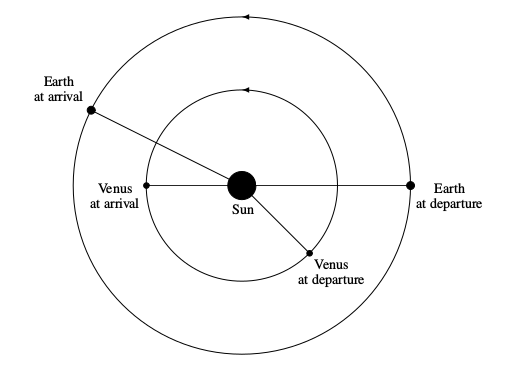
\includegraphics[width=0.5\textwidth]{prob5}}
%\put(2.6,-0.3){$\theta$}
%\put(-0.35,1.9){$M_e$}
%\put(3.5,2.5){$e=0$}
%\put(2.4,3.3){$e=0.8$}
%\end{picture}
%}
%
%\vspace*{1cm}
%Parts of the Matlab codes to generate the above plot are given at the next page.
%
%\begin{subprob}
%\item Complete the 2nd line at the next page such that the eccentricity $e$ is varied as $e=0,\,0.2,\,0.4,\,0.6,\,0.8$.
%\item Complete the 4th to 6th lines at the next page to compute $M_e$ and $E$ for each value of $\theta$.
%\item Discuss what would happen to the plot if the command \textit{hold on} at the 10th line is deleted.
%\end{subprob}
%
%\newpage
%{\Large\selectfont\renewcommand{\baselinestretch}{1.4}
%\begin{alltt}
%
% 1: figure;
% {\textbf{2}}: for e=
% 3:     theta=linspace(0,2*pi,501);
% \textbf{4}:     for k=1:
% \textbf{5}:        E 
% \textbf{6}:        Me
% 7:     end
% 8:     
% 9:     plot(theta,Me);
%\textbf{10}:     hold on;
%11: end
%\end{alltt}}
%
%\end{prob}
%
%
%\end{document}
%
%Consider a spacecraft in an elliptic orbit around the Earth.
%
%\vspace*{0.3cm}
%\centerline{
%\setlength{\unitlength}{2.0em}\centering\footnotesize
%\begin{picture}(8,6.4)(-4,-3.2)
%\put(0,0){\ellipse{8}{6.4}}
%\put(2.4,0){\circle*{0.8}}
%\put(-4,0){\line(1,0){8}}
%\put(-0.8,-0.3){$r_a$}
%\put(3.2,-0.3){$r_p$}
%\put(4,0){\circle*{0.15}}\put(4.2,0){$A$}
%\put(-4,0){\circle*{0.15}}\put(-4.5,0){$P$}
%\put(2.4,0){\line(0,1){2.56}}
%\put(2.4,2.56){\circle*{0.15}}\put(2.55,2.6){$D\;(\theta=\frac{\pi}{2})$}
%\put(2.4,0){\line(0,-1){2.56}}
%\put(2.4,-2.56){\circle*{0.15}}\put(2.55,-2.8){$C\;(\theta=-\frac{\pi}{2})$}
%\end{picture}}
%\vspace*{0.3cm}
%
%\noindent We observe that the maximum distance $r_a$, and the minimum distance $r_p$ to the center of the Earth are given by
%\begin{align*}
%r_a = 32000\,\mathrm{km},\qquad r_p = 8000\,\mathrm{km}.
%\end{align*}
%Assume that the gravitational parameter of the Earth is given by $\mu = 398,\!600\;\mathrm{km^3/s^2}$.
%
%\begin{subprob}
%\item Show that the eccentricity is $e=0.6$ and the period is $T=2.8148\times 10^{4}\,\mathrm{sec}$.
%\vspace*{2.5cm}
%\item Find the time required for the spacecraft to move from $A$ to $P$ through $D$, namely $t_{ADP}$ (specify the units).
%\vspace*{2.0cm}
%\item Find the time required for the spacecraft to move from $P$ to $C$, namely $t_{PC}$ (specify the units).
%\end{subprob}
%\end{prob}
%
%
%\end{document}
%
%
%\renewcommand{\theprob}{\arabic{prob} \textit{(15pt)}}
%\begin{prob}
%Mark whether each statement written in \textit{italic font} is True or False.
%\begin{subprob}
%%\item \textit{Newton's 2nd law of motion is satisfied for any reference frame}. [True, False]
%%\item \textit{The mutual gravitational potential between two point masses is proportional to the distance between them.} [True, False]
%
%%\item \textit{The orbital speed of the Mars around the Sun is greater than that of the Saturn.} [True, False]
%
%\item Consider the following two spacecraft, namely $A$ and $B$ on circular orbits. 
%The orbital radius and the mass of them are denoted by $r_A,m_A$, and $r_B,m_B$, respectively. Suppose that $r_B=2r_A$ and $m_B=1.5m_A$. Then, \textit{the gravitational potential energy of Spacecraft $A$ is greater than that of Spacecraft $B$}. [True, False]
%
%
%\vspace*{0.3cm}
%\centerline{
%\setlength{\unitlength}{2.5em}\centering\footnotesize
%\begin{picture}(3,3)(-1.5,-1.5)
%\put(0,0){\circle*{0.3}}
%\put(0,0){\circle{1.5}}
%\put(0,0){\circle{3}}
%\put(0.6495,0.3750){\circle*{0.06}}
%\put(1.5,0){\circle*{0.1}}
%\put(1.6,-0.3){$B$}
%\put(0.8,0.3){$A$}
%\put(3,-0.2){\shortstack[c]{$r_B=2r_A$\\$m_B=1.5m_A$}}
%\end{picture}}
%
%\item For the two spacecraft $A$ and $B$ shown above at the part (a), \textit{the orbital velocity of Spacecraft $A$ is greater than that of Spacecraft $B$, i.e. $v_A > v_B$}. [True, False]
%
%\item Two circular orbits, namely Orbit 1 and Orbit 2 are illustrated with respect to the geocentric equatorial frame as follows, where gray circles denote the Earth equatorial plane, and the blue circle and the green circle denote the orbital plane for Orbit 1 and Orbit 2, respectively. Note that spacecraft on Orbit 1 is rotating \underline{clockwise}, and spacecraft on Orbit 2 is rotating \underline{counterclockwise}. Then, \textit{the longitude of ascending node of Orbit 1 is greater than Orbit 2, i.e. $\Omega_1 > \Omega_2$.} [True, False]
%
%%\renewcommand{\thesubfigure}{}
%%\setlength{\unitlength}{0.1\textwidth}
%%\begin{figure}[h]
%%\centerline{\footnotesize
%%	\subfigure[Orbit 1]{\begin{picture}(2.2,2.25)(0,0.05)
%%	\put(0,0.395){\includegraphics[width=0.25\textwidth]{prob1c1}}
%%	\put(0.2,0.5){$\vec X$}
%%	\put(2.4,0.6){$\vec Y$}
%%	\put(1.25,2.3){$\vec Z$}
%%	\end{picture}}\hspace*{0.2\textwidth}
%%	\subfigure[Orbit 2]{\begin{picture}(2.2,2.25)(0,0.05)
%%	\put(0,0){\includegraphics[width=0.25\textwidth]{prob1c2}}
%%	\put(0.2,0.5){$\vec X$}
%%	\put(2.4,0.6){$\vec Y$}
%%	\put(1.25,2.3){$\vec Z$}
%%	\end{picture}}
%%}
%%\end{figure}
%
%\item For the two orbits illustrated above at the part (c), \textit{the inclination of Orbit 1 is greater than the inclination of Orbit 2, i.e., $i_1 > i_2$}. [True, False]\\
%(Hint: inclination is the angle between $\vec h$ and $\vec Z$).
%
%\item The Aitken basin is the largest crater on the far side of the Moon. The following two lunar orbits, namely Orbit 1 and Orbit 2 are proposed to generate a topographic map of the Aitken basin, which is denoted by $A$ below. The size and the shape of two orbits are identical, i.e., $a_1=a_2$, $e_1=e_2$, and $T_1=T_2$. Assume that the Moon is not rotating, so $A$ is stationary with respect to both orbits. Then, \textit{spacecraft on Orbit 1 can take images of $A$ for a longer time period per each revolution than another spacecraft on Orbit 2}. [True, False]
%
%\definecolor{dunkelmagenta}{rgb}{.3, 0, .3}
%
%
%\vspace*{0.3cm}
%\centerline{
%\setlength{\unitlength}{0.08\textwidth}\centering\footnotesize
%\begin{picture}(3,2)(-1.5,-1)
%\put(0,0){\circle*{0.4}}
%\put(1.0,0){\ellipse{3.0}{2}}
%{\filltype{white}
%\put(0.2,0.0){\circle*{0.06}}}
%\put(0.9,-1.2){\text{Orbit 2}}
%\put(0.25,0.05){$A$}
%\put(-0.25,-0.4){\text{Moon}}
%\put(1.0,-1){\vector(1,0){0}}
%\put(1.0,1){\vector(-1,0){0}}
%\color{blue}\put(-1.0,0){\ellipse{3.0}{2}}
%\put(-1.0,-1){\vector(1,0){0}}
%\put(-1.0,1){\vector(-1,0){0}}
%\put(-1.6,-1.2){\text{Orbit 1}}
%\end{picture}}
%\end{subprob}
%\end{prob}
%
%
%\clearpage\newpage
%\renewcommand{\theprob}{\arabic{prob} \textit{(15pt)}}
%
%\begin{prob}
%The position and the velocity of an asteroid heading toward a planet are measured with respect to an arbitrary $x-y$ frame as follows:
%\begin{align*}
%\vec r =[20,\; 15,\; 0]\,\mathrm{km}, \quad \vec v=[-6,\; 0,\; 0] \,\mathrm{km/s}.
%\end{align*}
%%
%\centerline{
%\setlength{\unitlength}{0.04\textwidth}\centering\footnotesize
%\begin{picture}(4,5)(0,-1)
%\put(0,0){\circle*{1}}
%\put(4,3){\circle*{0.2}}
%\put(-2,0){\vector(1,0){7}}
%\put(0,-1){\vector(0,1){5}}
%\put(0,0){\vector(4,3){3.9}}
%\put(4,3){\vector(-1,0){1}}
%\put(5,-0.3){$x$}
%\put(0.2,4){$y$}
%\put(2,1.1){$\vec r$}
%\put(3.5,3.1){$\vec v$}
%\put(-1.4,1.4){\circle*{0.1}}
%\put(-1.8,1.5){$P$}
%\put(0,0){\vector(-1,1){1.35}}
%\put(-1.2,0.5){$\vec r_p$}
%\put(0.5,-0.5){Planet}
%\put(4.2,3.1){Asteroid}
%\end{picture}}
%%
%We wish to determine whether it would hit the planet. The gravitational parameter of the planet is given by {$\underline{ \mu=400\,\mathrm{km^3/s^2}}$}, and the radius of the planet is $R_{\mathrm{planet}}=6\,\mathrm{km}$. 
%
%\begin{subprob}
%\item Find the specific energy $\mathcal{E}$ and the angular momentum $h$.
%\vspace*{3.5cm}
%\item Show that the eccentricity is given by $e=1.0966$, and ALSO show that the asteroid does not hit the planet, i.e., $r_p > R_{\mathrm{planet}}=6\,\mathrm{km}$.
%\vspace*{3.5cm}
%\item We wish to find the point where the asteroid is closest to the planet. Find the \underline{vector} $\vec r_p$ from the center of the planet to the periapsis $P$. 
%\end{subprob}
%
%\end{prob}
%
%
%\clearpage\newpage
%\renewcommand{\theprob}{\arabic{prob} \textit{(12pt)}}
%
%\begin{prob}
%A spacecraft is on a \underline{hyperbolic} orbit around the Mars, and it is designed to communicate with  the Mars rover. The orbital parameters and the location of the Mars rover are illustrated as follows. Due to the limitation of the radar, the spacecraft can maintain a communication link with the rover only between the points $A$ and $B$.
%
%\centerline{
%\setlength{\unitlength}{0.025\textwidth}\centering\footnotesize
%\begin{picture}(5,15.5)(0,-4.5)
%\put(0,0){\circle*{1.6}}
%\put(-2,0){\vector(1,0){11}}
%\put(0,-1){\vector(0,1){11}}
%\renewcommand{\xscale}{1}
%\renewcommand{\yscale}{1}
%\scaleput(0,0){\curve(%-1.8031,  -10.2256,
%%          0,   -8.4000,
%%    1.2247,   -6.9457,
%%    2.0876,   -5.7356,
%    2.7097,   -4.6933,
%    3.1630,   -3.7695,
%    3.4921,   -2.9302,
%    3.7256,   -2.1509,
%    3.8814,   -1.4127,
%    3.9708,   -0.7002,
%    4.0000,         0,
%    3.9708,    0.7002,
%    3.8814,    1.4127,
%    3.7256,    2.1509,
%    3.4921,    2.9302,
%    3.1630,    3.7695,
%    2.7097,    4.6933,
%    2.0876,    5.7356,
%    1.2247,    6.9457,
%         0,    8.4000,
%   -1.8031,   10.2256)}
%\scaleput(3.4921,-2.9302){\circle*{0.2}}   
%\scaleput(1.2247,6.9457){\circle*{0.2}}   
%\put(0,0){\curve(0,0,3.4921,-2.9302)}
%\put(0,0){\curve(0,0,1.2247,6.9457)}
%{\filltype{white}\put(0.7518,0.2736){\circle*{0.3}}}
%\put(0.9,0.3){Rover}
%\put(3.8,-3.4){$A,\;\theta_A=320^\circ$}   
%\put(1.4,7.2){$B,\;\theta_B=80^\circ$}   
%\put(10,3){\normalsize\shortstack[c]{$a=40,000\,\mathrm{km}$\\$h = 18,783\,\mathrm{km^2/s}$\\$\mu=42,000\,\mathrm{km^3/s^2}$}}
%\put(4,0){\circle*{0.2}}   
%\put(4.2,-0.6){$P$}
%\color{blue}
%\scaleput(0,0){\curve(%-1.8031,  -10.2256,
%%          0,   -8.4000,
%%    1.2247,   -6.9457,
%%    2.0876,   -5.7356,
%%    2.7097,   -4.6933,
%%    3.1630,   -3.7695,
%    3.4921,   -2.9302,
%    3.7256,   -2.1509,
%    3.8814,   -1.4127,
%    3.9708,   -0.7002,
%    4.0000,         0,
%    3.9708,    0.7002,
%    3.8814,    1.4127,
%    3.7256,    2.1509,
%    3.4921,    2.9302,
%    3.1630,    3.7695,
%    2.7097,    4.6933,
%    2.0876,    5.7356,
%    1.2247,    6.9457)}
%%         0,    8.4000,
%%   -1.8031,   10.2256)}   
%\end{picture}}
%
%\begin{subprob}
%\item Show that the eccentricity of this orbit is given by $e=1.1$. 
%\vspace*{3cm}
%\item Find the total time period available for communication, i.e., find the time $t_{AB}$ for the spacecraft to move from $A$ to $B$.\\
%(Hint: $\frac{1}{\parenth{\frac{\mu^2}{h^3} (e^2-1)^{3/2}}} = 39036\,\mathrm{sec}$).
%\end{subprob}
%
%\end{prob}
%
%
%\clearpage\newpage
%\renewcommand{\theprob}{\arabic{prob} \textit{(15pt)}}
%
%\begin{prob}
%The orbital elements for a spacecraft orbiting around the Earth are given as follows:
%\begin{align*}
%(e=0.8,\quad \theta=270^\circ,\quad i= 90^\circ,\quad \Omega = 180^\circ,\quad \omega=270^\circ).
%\end{align*}
%The following figure illustrates the geocentric equatorial frame and the Earth equatorial plane.
%
%\vspace*{0.8cm}
%\centerline{
%\setlength{\unitlength}{1.7em}\centering\footnotesize
%\begin{picture}(20,20)(-10,-7)
%\put(0,0){\ellipse{14}{3.0}}
%\put(0,0){\vector(1,0){9}}
%\put(0,0){\vector(0,1){9}}
%\put(0,0){\vector(-3,-2){4.0}}
%\put(-4.8,-2.9){$\vec X$}
%\put(9.2,-0.5){$\vec Y$}
%\put(0.2,8.7){$\vec Z$}
%\end{picture}}
%\vspace*{0.3cm}
%
%\vfill
%\noindent Sketch the orbit of this spacecraft according to the following steps.
%\begin{subprob}
%\item Draw the node vector $\vec N$, and specify the angle between $\vec N$ and $\vec X$. Mark the ascending node by a point $A$.
%\item Draw the orbital plane, and the direction of the angular momentum vector $\vec h$. Specify the angle between the orbital plane and the equatorial plane.
%\item Draw the eccentricity vector $\vec e$, and specify the angle between $\vec N$ and $\vec e$.
%\item Sketch the orbit. Mark the periapsis by a point $P$.
%\item Mark the location of the spacecraft on the orbit by a point $S$. 
%\end{subprob}
%
%\end{prob}
%
%
%\clearpage\newpage
%\renewcommand{\theprob}{\arabic{prob} \textit{(13pt)}}
%
%\begin{prob}
%The following diagram shows six orbits with the identical periapsis $r_p$, but with varying eccentricity. We wish to determine how the specific kinetic energy varies compared with the specific gravitational potential energy for these orbits. 
%
%%\centerline{\includegraphics[width=0.2\textwidth]{prob5a.eps}}
%
%\begin{subprob}
%\item The specific kinetic energy $K$ and the magnitude of the gravitational potential energy $|U|$ are given by
%\begin{align*}
%K= \frac{1}{2}v^2,\quad |U|=\frac{\mu}{r}.
%\end{align*}
%Recall that $r=\dfrac{h^2/\mu}{1+e\cos\theta}$, $v_r=\dfrac{\mu}{h}e\sin\theta$, and $v_\theta=\dfrac{\mu}{h}(1+e\cos\theta)$. Show that the ratio $\sigma$ of the kinetic energy to the gravitational potential energy is given by
%\begin{align}
%\sigma = \frac{K}{|U|} =  \frac{1+e^2+2e\cos\theta}{2(1+e\cos\theta)}
%\end{align}
%\vspace*{4cm}
%
%
%\item The following figure illustrates the ratio $\sigma$ over $-180^\circ<\theta<180^\circ$ for several values of the eccentricity $e$. \\
%
%%\centerline{\includegraphics[width=0.5\textwidth]{prob5b.eps}}
%
%\clearpage\newpage
%
%\setcounter{enumi}{1}
%\item\!(continued)\; Parts of the Matlab code that is used to generate this figure are given as follows. Complete the Matlab code. You DO NOT have to worry about the axis labels $\theta,\sigma$ or the color of lines. You MAY NOT have to use all of 15 lines.
%
%{\large\selectfont\renewcommand{\baselinestretch}{1.4}
%\begin{alltt}
% 1: clear all;
% 2: close all;
% 3: theta=linspace(-pi,pi,200);
% 4: \textcolor{blue}{for} e=0:0.2:1
% 5:     \textcolor{blue}{for} k=1:
% 6:         ratio
% 7:     
% 8:     plot(
% 9:     hold on;
%10:     
%11:
%12:
%13:
%14:
%15:
%\end{alltt}}
%\vspace*{0.3cm}
%
%\item Based on the above code and the equation (1), what is the value of the eccentricity $e$ corresponding to the red curve at the figure.
%
%\end{subprob}
%	
%	
%\end{prob}
%
%\end{document}
%
%\item \textit{The angle between the orbital plane and and the Earth equatorial plane is defined by the orbital element $\Omega$.} [True, False]
%%\item \textit{The unit of a gravitational parameter $\mu$ is \textbf{\textit{always}} $\mathrm{km^3/s^2}$}. [True, False]
%\item Consider the following two orbits around the Earth: a circular orbit (solid line) and an elliptic orbit (dotted line). 
%
%\vspace*{0.3cm}
%\centerline{
%\setlength{\unitlength}{2.5em}\centering\footnotesize
%\begin{picture}(6,5.0)(0.0,-0.5)
%%\put(0,0){\includegraphics[width=0.3\textwidth]{prob1c1.eps}}
%\put(4.5,2.212){\line(1,0){1.05}}
%\put(4.5,1.9){$r=r_p$}
%\end{picture}}
%
%
%As shown above, the distance to the periapsis of the elliptic orbit, namely   $r_p$ is equal to the radius of the circular orbit $r$. \textit{Then, the angular momentum of the elliptic orbit $h_{e}$ is greater than the angular momentum of the circular orbit $h_{c}$, i.e. $h_e > h_c$.} [True, False]
%
%\item Between the above two orbits, the specific energy of the elliptic orbit $\mathcal{E}_e$ is larger than the specific energy of the circular orbit $\mathcal{E}_c$, i.e. $\mathcal{E}_e > \mathcal{E}_c$. [True, False]
%\end{subprob}
%\end{prob}
%
%\clearpage\newpage
%\renewcommand{\theprob}{\arabic{prob} \textit{(15pt)}}
%\begin{prob}
%We consider a planar motion of two masses acting under their mutual gravitational potential. A mass $m_1$ is initially at rest with respect to an inertial frame. Another mass $m_2$ is moving with a velocity $V$ as follows:
%
%\centerline{
%\setlength{\unitlength}{2.2em}\centering\footnotesize
%\begin{picture}(6,5.0)(0.0,-0.5)
%\put(0,0){\vector(1,0){6}}
%\put(0,0){\vector(0,1){4}}
%\put(0,0){\circle*{0.6}}
%\put(4,0){\circle*{0.3}}
%\put(6,-0.2){$x$}
%\put(-0.3,4){$y$}
%\put(0.4,-0.3){$m_1$}
%\put(4.2,-0.3){$m_2$}
%\put(4.1,2){$V$}
%\linethickness{0.8pt}
%\put(4,0){\vector(0,1){2}}
%\end{picture}}
%
%\noindent More explicitly, the initial position vector and the initial velocity vector of $m_1$, $m_2$ in the inertial frame are given by
%\begin{align*}
%\vec R_1(0) = \begin{bmatrix} 0 \\ 0\end{bmatrix}\,\mathrm{m},\quad \dot {\vec R}_1(0)=\begin{bmatrix} 0 \\ 0\end{bmatrix}\,\mathrm{m/s},\qquad\qquad
%\vec R_2(0) = \begin{bmatrix} 1 \\ 0\end{bmatrix}\,\mathrm{m},\quad \dot {\vec R}_2(0)=\begin{bmatrix} 0 \\ V\end{bmatrix}\,\mathrm{m/s}.
%\end{align*}
%Assume that $m_1=2\,\mathrm{kg}$, $m_2=1\,\mathrm{kg}$, \underline{$\mu=1\,\mathrm{m^3/s^2}$}.
%
%\begin{subprob}
%\item Suppose that $V=1\,\mathrm{m/s}$. What is the location of the mass center $\vec R_G$ at $t=3$ seconds (specify the units).
%\vspace*{3.5cm}
%\item Suppose that $V=1\,\mathrm{m/s}$. What is the type of the orbit for the relative motion $\vec r = \vec R_2 -\vec R_1$.\\
%(Hint: compute $\mathcal{E}$ and $h$, then use the following equation to determine $e$, $\quad\mathcal{E}=-\frac{1}{2} \frac{\mu^2}{h^2}(1-e^2)$.)
%\vspace*{5.5cm}
%\item What is the minimum value of $V$ that makes the distance between two masses approaches infinity, i.e. a parabolic orbit (specify the units).
%\end{subprob}
%\end{prob}
%
%\clearpage\newpage
%\renewcommand{\theprob}{\arabic{prob} \textit{(20pt)}}
%
%\begin{prob}
%Consider a spacecraft in an elliptic orbit around the Earth.
%
%\vspace*{0.3cm}
%\centerline{
%\setlength{\unitlength}{2.0em}\centering\footnotesize
%\begin{picture}(8,6.4)(-4,-3.2)
%\put(0,0){\ellipse{8}{6.4}}
%\put(2.4,0){\circle*{0.8}}
%\put(-4,0){\line(1,0){8}}
%\put(-0.8,-0.3){$r_a$}
%\put(3.2,-0.3){$r_p$}
%\put(4,0){\circle*{0.15}}\put(4.2,0){$A$}
%\put(-4,0){\circle*{0.15}}\put(-4.5,0){$P$}
%\put(2.4,0){\line(0,1){2.56}}
%\put(2.4,2.56){\circle*{0.15}}\put(2.55,2.6){$D\;(\theta=\frac{\pi}{2})$}
%\put(2.4,0){\line(0,-1){2.56}}
%\put(2.4,-2.56){\circle*{0.15}}\put(2.55,-2.8){$C\;(\theta=-\frac{\pi}{2})$}
%\end{picture}}
%\vspace*{0.3cm}
%
%\noindent We observe that the maximum distance $r_a$, and the minimum distance $r_p$ to the center of the Earth are given by
%\begin{align*}
%r_a = 32000\,\mathrm{km},\qquad r_p = 8000\,\mathrm{km}.
%\end{align*}
%Assume that the gravitational parameter of the Earth is given by $\underline{\mu = 400,\!000\;\mathrm{km^3/s^2}}$.
%
%\begin{subprob}
%\item Find the eccentricity $e$ and the semi-major axis $a$ (specify the units).
%\vspace*{2.0cm}
%\item Find the specific energy $\mathcal{E}$ and the angular momentum $h$ (specify the units).
%\vspace*{2.0cm}
%\item Find the period $T$, and the time required for the spacecraft to move from $A$ to $P$ through $D$, namely $t_{ADP}$ (specify the units).
%\vspace*{2.0cm}
%\item Find the time required for the spacecraft to move from $C$ to $D$ through $A$, namely $t_{CAD}$ (specify the units).
%\end{subprob}
%\end{prob}
%
%%\clearpage\newpage
%%\begin{prob}
%%Consider a Molniya-type orbit that has an inclination of $i=63.43^\circ = 1.107\,\mathrm{rad}$. We have
%%\begin{align*}
%%T=12\,\mathrm{hours}=43200\,\mathrm{sec}, \quad \omega=-90^0=-\frac{\pi}{2}\,\mathrm{rad},\quad    \vec h = [0, -55266, 27643]\,\mathrm{km^2/s}.
%%\end{align*}
%%Assume $\mu = 398600\,\mathrm{km^3/s^2}$. We wish to determine the position vector to the apoapsis $\vec r_a$. 
%%
%%\begin{subprob}
%%\item Find the semimajor axis $a$ and the specific angular momentum $h$ (specify the unit).
%%\vspace*{2.5cm}
%%\item Find the eccentricity $e$ (specify the unit).
%%\vspace*{2.0cm}
%%\item Find the longitude of the ascending node $\Omega$ from $\vec h$ (specify the unit).
%%\vspace*{2.0cm}
%%\item Find $\hat N$ and $\hat N_t$  (specify the unit).
%%\vspace*{2.5cm}
%%\item What is the true anomaly $\theta$ at the apoapsis. Find $\hat u_r$ (specify the unit).
%%\vspace*{2.5cm}
%%\item Find $r_a$ and $\vec r_a$ (specify the unit).
%%\vspace*{2.5cm}
%%\end{subprob}
%%
%%\end{prob}
%
%
%\clearpage\newpage
%\renewcommand{\theprob}{\arabic{prob} \textit{(15pt)}}
%
%\begin{prob}
%The orbital elements for a spacecraft orbiting around the Earth is given as follows
%\begin{align*}
%(e=0.6,\quad \theta=270^\circ,\quad i= 90^\circ,\quad \Omega = 45^\circ,\quad \omega=180^\circ).
%\end{align*}
%The following figure illustrates the geocentric equatorial frame and the Earth equatorial plane.
%
%\vspace*{0.8cm}
%\centerline{
%\setlength{\unitlength}{1.7em}\centering\footnotesize
%\begin{picture}(20,20)(-10,-12)
%\put(0,0){\ellipse{14}{3.0}}
%\put(0,0){\vector(1,0){9}}
%\put(0,0){\vector(0,1){9}}
%\put(0,0){\vector(-3,-2){4.0}}
%\put(-4.8,-2.9){$\vec X$}
%\put(9.2,-0.5){$\vec Y$}
%\put(0.2,8.7){$\vec Z$}
%\end{picture}}
%\vspace*{0.3cm}
%
%\vfill
%\noindent Sketch the orbit of this spacecraft according to the following steps.
%\begin{subprob}
%\item Draw the node vector $\vec N$, and specify the angle between $\vec N$ and $\vec X$. Mark the ascending node by a point $A$.
%\item Draw the orbital plane, and the direction of the angular momentum vector $\vec h$. Specify the angle between the orbital plane and the equatorial plane.
%\item Draw the eccentricity vector $\vec e$, and specify the angle between $\vec N$ and $\vec e$.
%\item Draw the orbit. Mark the periapsis by a point $P$.
%\item Mark the location of the spacecraft on the orbit by a point $S$. 
%\end{subprob}
%
%\end{prob}
%
%
%\clearpage\newpage
%\begin{prob}
%In a sun-synchronous orbit, the average precession rate of $\Omega$ is the same as the orbital angular rate of the Earth around the Sun:
%\begin{align}
%\dot{\overline \Omega} = -\bracket{\frac{3}{2} \frac{\sqrt{\mu} J_2 R_E^2}{(1-e^2)^2 }}\frac{\cos i}{a^{7/2}} = 2\pi \,(\mathrm{rad/year}) = 2.0\times 10^{-7} (\mathrm{rad/sec}),
%\end{align}
%where ${\mu = 400,\!000 \,\mathrm{km^3/s^2}}$, ${R_E=6400\,\mathrm{km}}$, ${J_2 = 0.00108}$. In this question, we only consider \underline{circular} sun-synchronous orbits. Therefore, the eccentricity is given by $e=0$, and the semimajor axis $a$ is equal to the orbital radius. Substituting these into (1), we obtain
%\begin{align}
%\dot{\overline \Omega}= -4.2\times 10^7\times\frac{\cos i}{a^{7/2}} = 2.0\times 10^{-7}\,(\mathrm{rad/sec}).
%\end{align}
%
%\begin{subprob}
%\item From (2), find the value of the inclination $i$ that maximizes the orbital radius $a$ of circular sun-synchronous orbits. Show that the corresponding maximum orbital radius, namely $a_M$, is given by $\underline{a_M=12361\,\mathrm{km}}$.
%\vspace*{2.5cm}
%
%\item Show that the inclination $i$ and the orbital radius $a$ of circular sun-synchronous orbits satisfy
%\begin{align}
%\cos i = - \parenth{\frac{a}{a_M}}^{7/2}.\label{eqn:i}
%\end{align}
%\vspace*{2.5cm}
%
%
%
%\item Write a Matlab function, namely \texttt{SunSync.m} that returns the inclination $i$ satisfying \refeqn{i} for a given orbital radius $a$.\\ (Input variable: \texttt{a}, Output variable: \texttt{i}, Function name: \texttt{SunSync}).
%
%{\large\selectfont\renewcommand{\baselinestretch}{1.4}
%\begin{verbatim}
%1: function [
%2: aM=12361;
%3:
%4:
%5:
%\end{verbatim}}
%
%
%
%
%\newpage
%\item Write Matlab scripts to draw the following figure that represents the relationship between the inclination $i$ and the orbital radius $a$ of circular sun-synchronous orbits. You may use the matlab function \texttt{SunSync} defined at part (c).\\
%
%\centerline{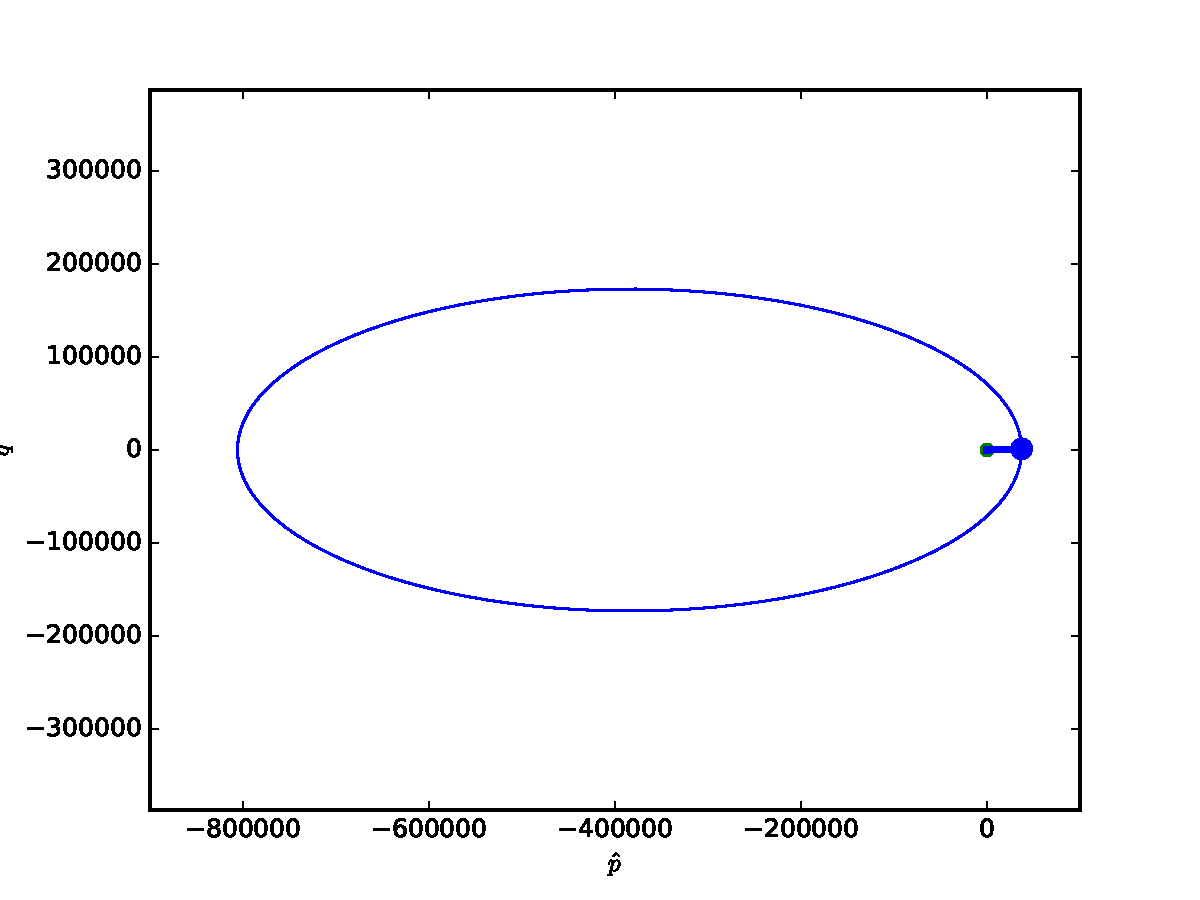
\includegraphics[width=0.5\textwidth]{prob4.eps}}
%
%{\large\selectfont\renewcommand{\baselinestretch}{1.4}
%\begin{verbatim}
% 1: clear all;
% 2: close all;
% 3: a=linspace(6400,12361,
% 4: for k=1:
% 5:
% 6:
% 7:
% 8:
% 9:
%10:
%11:
%12:
%13:
%14:
%15:
%\end{verbatim}}
%
%
%
%
%\end{subprob}
%\end{prob}
%
%
%
%

\end{document}

),